\chapter{Supersymmetry}
\label{chap:susy}
Supersymmetry was originally developed out of an attempt to understand why all particle interactions seem to obey Poincar{\'e} symmetries, but not all interactions allowed by the Poincar{\'e} group are are manifest in nature \cite{Golfand:1971iw, Wess:1974tw}. The idea that a larger symmetry may exist, one that governs which interactions are allowed and which are not, was a prevailing source of curiosity at the time, and remains so today. 

Because the ten generators of the Poincar{\'e} group have been mapped to the non-spin related spacetime symmetries (four translations, three rotations, and three boosts), it is natural to suppose that any larger symmetry containing the Poincar{\'e} group should involve the only remaining degrees of freedom, namely spin. Such a symmetry, which is called a supersymmetry, would generate transformations that shift quantum states by a fundamental unit of spin, $\hbar$/2, modeled as the action of an operator $\hat{Q}$ such that
\begin{equation}
\label{eq:SusyOperators}
\hat{Q}\ket{\text{boson}}=\ket{\text{fermion}},\text{\ \ \ } \hat{Q}\ket{\text{fermion}}=\ket{\text{boson}}.
\end{equation}
Since the $\ket{\text{boson}}$ and $\ket{\text{fermion}}$ states differ by a spin of $\hbar$/2, conservation of angular momentum requires that the operator $\hat{Q}$ itself carry spin $\hbar$/2, and so $\hat{Q}$ is identified as a fermionic operator obeying the fermion anti-commutation relations
\begin{equation}
\acomm{\hat{Q}_\alpha}{\hat{Q}_{\dot{\beta}}^\dag}=-2\sigma^{\mu}_{\alpha \dot{\beta}}\hat{P}_\mu,\\
\end{equation}
\begin{equation}
\acomm{\hat{Q}_\alpha}{\hat{Q}_{\beta}}=0,\ \ \  \acomm{\hat{Q}_{\dot{\alpha}}^\dag}{\hat{Q}_{\dot{\beta}}^\dag}=0.\footnote{Here, $\hat{P}_\mu$ is the generator of momentum translations, $\sigma^\mu$ is a four-vector of SU(2) rotation generators (Pauli matrices), and $\alpha$ and $\beta$ denote spinor indexes.}
\end{equation}
The pair of states in (\ref{eq:SusyOperators}), $\ket{\text{boson}}$ and $\ket{\text{fermion}}$, form a single object called a supermultiplet, where the fermion state is considered to be a field and the boson state is the corresponding ``superfield'', or vice versa. As with all QFTs, the fields are quantized,  and each field begets a particle that carries the quantum numbers of the field. Thus, in a supersymmetric framework, there are always two particles, dubbed ``superpartners'', that are identical copies of each other\textemdash except for their spin, of course, which differs by a fundamental increment. In particular, since $\hat{Q}$ commutes with the gauge generators of the theory as well as the momentum generator,
\begin{equation}
\comm{\hat{Q}_{\alpha}}{\hat{T}^\mu}=0,\text{\ \ \ }\comm{\hat{Q}_\alpha}{\hat{P}^\mu}=0,
\end{equation}
the particle and superpartner possess the same charges under all gauge groups and also have the same mass. 

In a Lagrangian obeying supersymmetry, the terms involving the superfields only carry model parameters that appear in the non-supersymmetric portion of the Lagrangian. This means that all couplings, mixing angles, and masses associated with the superfields are either already set by the gauge symmetries, or can be measured once and for all through experiments that probe the non-supersymmetric sector of the theory. This is true, however, only if $\SUSY$ is an unbroken symmetry. As we'll learn shortly, if the laws of physics do exhibit any $\SUSY$ at all, it must be a broken $\SUSY$, at least at low energies close the vacuum state.

\section{Supersymmetry in our universe}

It was not until some time after its conception that $\SUSY$ began to be viewed as an idea to be taken seriously.  The idea became popular when it was learned that supersymmetry could potentially solve the hierarchy problem. The unnaturally small $\sm$ VEV receives large corrections from each boson and fermion that interacts with the vacuum (Section \ref{sec:finetune}). But there is some relief, or possibly a clue, in the fact that the bosons and fermions contribute with the opposite sign (compare \ref{eq:FermLoop} and \ref{eq:ScalarLoop}). If each $\sm$ fermion were to be paired with an equivalent boson and vice versa, the quadratic VEV corrections would all cancel, and the smallness of the VEV would be a consequence of symmetry.

Indeed, a supersymmetric framework would yield a set of particles that automatically induces this cancelation. Where each $\sm$ field generates a huge correction to the VEV,  the corresponding superfield would generate the opposite huge correction, resulting in no net change to the electroweak breaking scale (see Fig. \ref{fig:SusyCancelations}). Supersymmetry could be the mechanism to explain nature's unusual mass pattern.

\begin{figure}[h]
\makebox[\textwidth][c]{
\centering
\subfloat[]{
  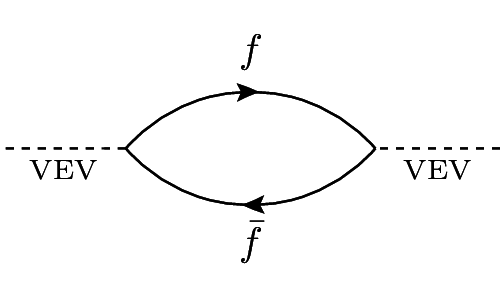
\includegraphics[width=0.5\linewidth]{figures/SM/VevFermionLoop.png}
}
\subfloat[]{
  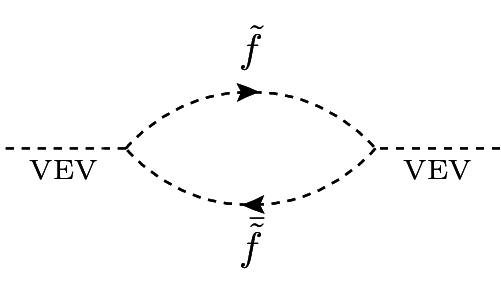
\includegraphics[width=0.5\linewidth]{figures/SUSY/VevSfermionLoop.png}
}
}
\caption{The cancelation.} 
\label{fig:SusyCancelations}
\end{figure}

But before $\SUSY$ can be seriously considered as a potential candidate, we must deal with the fact that the viability of a supersymmetric hypothesis in our universe faces two serious obstacles. They are:
\begin{enumerate}
\item{A supersymmetric $\sm$ could result in the proton being unstable.}
\item{Supersymmetry has not been observed in any experiment before.}
\end{enumerate}
Perhaps it is best to deal with these one by one.

\noindent
1. If supersymmetric interactions existed, protons would quickly decay because $\SUSY$ introduces interactions that break the accidental $\sm$ symmetries that conserve baryon and lepton numbers. Two quarks inside the proton could annihilate to form a lepton superpartner (slepton), and the proton would fly to pieces after a period of a few seconds to a year. However, experiments \cite{Miura:2009yma} have determined that the proton lifetime is greater than $10^{32}$ years, so clearly there is a spectacular discrepancy to be resolved. The situation can most easily be remedied by introducing an additional $\ztwo$ symmetry called $R$-parity \cite{Farrar:1982te}, which, as shown in Section \ref{sec:withztwo}, requires that superpartners always be produced or annihilate in pairs. This forbids the vertices involved in the proton's decay, thereby preserving proton stability. It should be noted that $R$-parity is not simply an ad hoc symmetry, but arises naturally out of many grand unification theories like SO(10), as well as out of continuous gauge symmetries that conserve B$-$L.

\noindent
2. If the $\sm$ exhibited an unbroken $\SUSY$, the masses of the superpartners would be identical to the masses of $\sm$ particles, and the superpartner of the electron would have been discovered perhaps a century ago. Supersymmetry has not been observed in any experiment so far; therefore, in order to be a viable hypothesis, it must be that the superpartners are much heavier than their $\sm$ counterparts, somehow. This can be arranged, so long as $\SUSY$ is a so-called ``softly'' broken symmetry, meaning that a certain set of terms can be added to the Lagrangian that violate $\SUSY$ by giving extra mass to the superpartners.

The fact that $\SUSY$ must be broken should not be taken as a strike against the hypothesis; as discussed in Section \ref{chap:SM}, the $\sm$ is already host to a very important symmetry that happens to be broken, namely, the electroweak $U(1)\times SU(2)$ symmetry.

As stated, even a broken $\SUSY$ will cure the $\sm$'s hierarchy problem, as long as the $\SUSY$ is only broken by a certain class of terms. Generically, these terms are of the form

\begin{equation}
\mathcal{L}_{SOFT}={\color{red}-\frac{1}{2}M_a\tilde{\lambda}_a\tilde{\lambda}_a}
{\color{Green}-\frac{1}{6}b_{ijk}\tilde{f}_i\tilde{f}_{j}\phi_k}
{\color{blue}-\frac{1}{2}b_{ij}\tilde{f}_i\tilde{f}_j}
{\color{orange}-m^2_{ij}\tilde{f}_{j}^*\tilde{f}_i}.
\label{eq:SoftBreak}
\end{equation}
The $\tilde{\lambda}$'s are the superpartner fields of gauge bosons (gauginos), the $\tilde{f}$'s are the superpartner fields of fermions (sfermions), and the $\phi$'s are scalar fields; repeated indices within a term imply a summation over species. The red and blue terms are responsible for endowing the superpartners with mass, and are needed to explain why $\SUSY$ so far has never been observed, solving problem 2. The green terms indicate the scalar trilinear interactions, and the orange are called the non-holomorphic terms~\cite{Peskin:1995ev}, which don't play a large role in this investigation but are included for completeness. I'll now explain how $\SUSY$, along with this generic set of soft breaking terms, could be realized in the the context of the $\sm$.

\section{The MSSM}
\label{sec:mssm}
Introducing supersymmetry into the $\sm$ yields the set of supermultiplets listed in Table \ref{tab:MSSM}. You'll notice that there are two Higgs supermultiplets. The reason, in short, is that $\SUSY$ requires there to be a second Higgs doublet to prevent an electroweak gauge anomaly \cite{Martin:1997ns}. Represented here are the fields that make up the minimal supersymmetric $\sm$ (MSSM), which predicts the existence of 41 extra fields in addition the 33 fields of the $\sm$. That is 33 superfields matching to the known $\sm$ fields, and eight new fields arising from the second Higgs doublet. The supersymmetric Lagrangian containing these fields is given by
\begin{align}
W_{MSSM}=\bar{u}\textbf{y$_d$}QH_u-\bar{d}\textbf{y$_d$}QH_d-\bar{e}y_eLH_d+\mu H_uH_d.
\end{align}

Table \ref{tab:MSSM} summarizes the fields of the MSSM before symmetry breaking.
\begin{table}
\centering
\caption{The supermultiplets of the MSSM. }
\begin{tabular}{  l | c | c | c | c}
\hline
\hline
Supermultiplets & spin 0 & spin 1/2 & spin 1 & number of fields/2 \\
\hline
\multirow{2}{*}{Higgs, Higgsino} & $H_u$  & $\tilde{H}_u$ &  & 2 \T\B\\
& $H_d$ & $\tilde{H}_{d}$ &  & 2 \T\B\\ 
\hline
& $\tilde{Q}_L$ & $Q_L$ &  & 6 \T\B\\
quark, squark& $\tilde{u}_{R}^*$ & $u_{R}^\dag$ &  & 3 \T\B\\
& $\tilde{d}_{R}^*$ & $d_{R}^\dag$ &  & 3 \T\B\\
\hline
\multirow{2}{*}{lepton, slepton} & $\tilde{L}_L$ & $L_L$ &  & 6 \T\B\\
& $\tilde{e}_{R}^*$ & $e_{R}^\dag$ &  & 3 \T\B\\
\hline
B boson, bino &  & $\tilde{B}$ & $B$ & 1 \T\B\\
W boson, wino &  & $\tilde{W}$  & $W$ & 3 \T\B\\
gluon, gluino &  & $\tilde{g}$ & $g$ & 8 \T\B\\
\hline
\hline
\end{tabular}
\label{tab:MSSM}
\end{table}
As discussed, an unbroken supersymmetric $\sm$ doesn't exist. Therefore, to complete the description of the MSSM, the generic soft-breaking Lagrangian in Equation \ref{eq:SoftBreak} must be expressed in terms of the specific superfields listed in Table \ref{tab:MSSM}. Suppressing the chirality labels, one obtains
\begin{equation}
\begin{split}
\mathcal{L}_{\text{SOFT},\,\text{MSSM}}=
&{\color{red}-1/2(M_1\tilde{B}\tilde{B}+M_2\tilde{W}\tilde{W}+M_3\tilde{g}\tilde{g})}\\
&{\color{Green}-\tilde{\bar{u}}\hat{\textbf{a}}_u\tilde{Q}H_u-\tilde{\bar{d}}\hat{\textbf{a}}_d\tilde{Q}H_d-\tilde{\bar{e}}\hat{\textbf{a}}_e\tilde{Q}H_d}\\
&{\color{blue}-\tilde{Q}^\dag\hat{\textbf{m}}_{Q}^2\tilde{Q}-\tilde{L}^\dag\hat{\textbf{m}}_{L}^2\tilde{L}-\tilde{\bar{u}}\hat{\textbf{m}}_{u}^2\tilde{\bar{u}}^\dag-\tilde{\bar{d}}\hat{\textbf{m}}_{d}^2\tilde{\bar{d}}^\dag}\\
&{\color{blue}-\tilde{\bar{e}}\hat{\textbf{m}}_{e}^2\tilde{\bar{e}}^\dag-bH_uH_d}\\
&{\color{orange}-m^2_{H_u}H_u^*H_u-m_{H_d}^2H_d^*H_d},
\end{split}
\label{eq:SoftBreakMSSM}
\end{equation}
where the bold hatted symbols are complex $3\times3$ matrices in family space, and colors show the correspondence between similar terms in Equations \ref{eq:SoftBreak} and \ref{eq:SoftBreakMSSM}. In total, Equation \ref{eq:SoftBreakMSSM} contains 107 unknown parameters \cite{Dimopoulos:1995ju}, which along with the four parameters from the second Higgs doublet, span the 111 unknown free parameters of the MSSM. That is 111 new parameters that must in principle be measured in future experiments, if the MSSM is indeed a model that describes nature.

Unfortunately, the large number of free parameters renders the MSSM parameter space impossible to explore exhaustively, at least for now. But, the vast set of experimental observations collected at particle physics experiments over decades, as well as theoretical motivations, can be used to constrain the model space, and make studying the MSSM a possibility. A number of constrained submodels of the MSSM have been developed and studied, two of which are discussed now.

\section{The cMSSM}
The constrained MSSM, or cMSSM \cite{Wess:1984jr}, is a well-named submodel of the MSSM that makes many assumptions about the MSSM. This reduces enormously the dimensionality of the model. Sufficient assumptions are made to reduce the number of $\SUSY$ breaking parameters from 107 to just five. Central to these defining assumptions is the idea that at some energy near the GUT scale ($10^{16}$ GeV), the superpartners become mass degenerate, a feature motivated by certain grand unification scenarios. This allows for all the sfermion masses to be set to a single value at the selected high energy, and the same for the gaugino and Higgsino masses, that is,
\begin{align}
{\color{red}M_3}={\color{red}M_2}={\color{red}M_3} & \equiv m_{1/2},\\
{\color{blue}\hat{\textbf{m}}_Q^2}={\color{blue}\hat{\textbf{m}}_L^2}={\color{blue}\hat{\textbf{m}}_u^2}={\color{blue}\hat{\textbf{m}}_d^2} ={\color{orange}m_{H_u}^2\mathds{1}}={\color{orange}m_{H_d}^2\mathds{1}}& \equiv m_0^2\mathds{1},\\
{\color{Green}\hat{\textbf{a}}_{u,d,e}} & \equiv A_0\cdot{\color{cyan}y_{t,b,\tau}} \eightZeroMat,\\
{\color{blue}b} & \equiv B_0\cdot \text{sign}(\mu).
\end{align}
The five black symbols on the right hand side, $m_{1/2}$, $m_0$, $A_0$, $B_0$, and sign($\mu$) are the
free parameters of the cMSSM, and the cyan $y_{t,b,\tau}$ are the known $\sm$ values of weak hypercharge for the top quark, bottom quark, and tau lepton. Because most of these are matrix equations, there are many more constraints than equations; 102 constraints to be specific. As mentioned, the cMSSM has very low dimensionality, and as a result, the model can be readily used to interpret experimental data. However, most of the constraints responsible for the reduction in dimensionality are not particularly well motivated, as they amount to assumptions about the laws of physics at scales that have never been observed by humans. Furthermore, any conclusions made about the cMSSM based on data collected in particle experiments are highly contingent, since only a tiny fraction of the phenomenological possibilities within the MSSM are realized in the cMSSM.

This is not to say that models like the cMSSM have not played an important role in the evolution of our understanding of $\SUSY$. They have provided benchmarks against which to compare the past and present sensitivity of experiments that probe supersymmetric hypotheses. They may play an increasingly important role in the future, if a significant part of the superpartner spectrum is discovered, and hints of the true $\SUSY$ breaking mechanism begins to appear. Such a breaking scheme could be quite elegant, described by only a few independent parameters. That said, very constrained models that make many untested assumptions are less useful when, as yet, there is absolutely no hint of supersymmetry.

\section{The pMSSM}
\label{sec:pmssm}
The phenomenological MSSM (pMSSM) is another submodel of the MSSM, one based on far fewer assumptions than the cMSSM. In particular, the pMSSM makes no assumption about how the $\SUSY$ breaking parameters are related at the GUT scale. The pMSSM~\cite{Berger:2008cq} was developed with the aim of making as few assumptions about the MSSM as possible, while reducing the size of the model's parameter space to a level that is practicable and workable. The assumptions defining the pMSSM are:
\begin{itemize}
\item{there are no new flavor changing neutral currents;}
\item{there are no new sources of CP violation at tree level;}
\item{the first and second generation fermions masses are degenerate, and}
\item{the lightest of the superpartners is the neutralino.}
\end{itemize}
The first two assumptions are motivated by the observation that CP-violating processes are extremely rare, even at loop level (higher order than tree-level), and flavor changing neutral currents are not observed at all. The third assumption is borne of the expectation that a model with two independent fermion generations will be as phenomenologically complete as a model with three generations, particularly in the early phases of discovery when only part of the full superpartner spectrum has been detected. The final assumption ensures that the lightest superpartner is electrically neutral, which is strongly motivated by cosmological observations. This leaves the following 19 parameters free:
\begin{itemize}
\item{three gaugino mass parameters {\color{red}$M_1$}, {\color{red}$M_2$}, and {\color{red}$M_3$};}
\item{one higgsino mass parameter $\mu$ and one pseudo-scalar Higgs mass $m_A$;}
\item{ten sfermion mass parameters {\color{blue}$m_{\tilde{f}}$}, where $\tilde{f}=\tilde{Q}_1$, $\tilde{U}_1$, $\tilde{D}_1$, $\tilde{L}_1$,  $\tilde{Q}_3$, $\tilde{U}_3$, $\tilde{D}_3$, $\tilde{L}_1$, and $\tilde{E}_3$ (imposing $m_{\tilde{Q}1}=m_{\tilde{Q}2}=m_{\tilde{L}1}=m_{\tilde{L}2}$);}
\item{three trilinear couplings {\color{Green}$A_t$}, {\color{Green}$A_b$}, and {\color{Green}$A_\tau$}, and}
\item{the ratio of the two Higgs vacuum expectation values $\text{tan}(\beta)=\text{VEV}_A/\text{VEV}_h$.}
\end{itemize}
With the particle masses free to vary independently throughout the model space, the pMSSM captures most of the possible, experimentally relevant phenomenology of the MSSM.  Despite the still rather large dimensionality of 19 free parameters, the model has been successfully used for the interpretation of experimental results, as demonstrated in ``The pMSSM interpretation of CMS 7 and 8 TeV results'' \cite{Khachatryan:2016nvf}, as well as in \cite{Carena:2012he, Aad:2015baa}. An detailed account is given in Chapter \ref{chap:run1pmssm}.

\section{Dark matter candidate}
If $\SUSY$ is realized in Nature in the context of the $\sm$, and if $R$-parity is conserved, there exists a new heavy stable particle, called the LSP (lightest supersymmetric particle). If this particle is electrically neutral and colorless, it matches the criteria necessary to be dark matter. There are several such candidates, including the superpartners of Higgs boson, the Z boson, and the photon. This possibility serves as an additional motivation for searching for $\SUSY$ in particle colliders. 
